\documentclass[12pt,letterpaper]{article}
%\usepackage[utf8]{inputenc}
\UseRawInputEncoding
\usepackage[english]{babel}
\usepackage{listings}
\usepackage{xcolor}
\usepackage{graphicx}

%For syntax highlighting
\definecolor{codegreen}{rgb}{0,0.6,0}
\definecolor{codegray}{rgb}{0.5,0.5,0.5}
\definecolor{codepurple}{rgb}{0.58,0,0.82}
\definecolor{backcolour}{rgb}{1,1,1}

%%Sets different parameters
\lstdefinestyle{mystyle}{
    backgroundcolor=\color{backcolour},   
    commentstyle=\color{codegreen},
    keywordstyle=\color{magenta},
    numberstyle=\tiny\color{codegray},
    stringstyle=\color{codepurple},
    basicstyle=\ttfamily\footnotesize,
    breakatwhitespace=false,         
    breaklines=true,                 
    captionpos=b,                    
    keepspaces=true,                 
    numbers=left,                    
    numbersep=5pt,                  
    showspaces=false,                
    showstringspaces=false,
    showtabs=false,                  
    tabsize=4
}
\lstset{style=mystyle}

\title{\textbf{Department of Computer Science and Engineering}}
\author{\textbf{Shivanirudh S G, 185001146, Semester VII }}

\date{15 July 2021}

\begin{document}
\maketitle
\hrule
\section*{\center{UCS1712 - Graphics and Multimedia Lab}}
\hrule 
\bigskip\bigskip

%Assignment name
\subsection*{\center{\textbf{Exercise 1: Study of Basic Output Primitives in C++ using OpenGL}}}

%Objective
\subsection*{\flushleft{Aim:}}
\begin{flushleft}
    To create an output window using OPENGL and to draw the following basic output primitives: POINTS, LINES, LINE\_STRIP, LINE\_LOOP, TRIANGLES, QUADS, QUAD\_STRIP, POLYGON.    
\end{flushleft}

%Code
\subsection*{\flushleft{Code:}}
\textbf{Common files}
\begin{flushleft}
\lstinputlisting[language = C++]{./Basics/Headers.h}
\lstinputlisting[language = C++]{./Basics/Signatures.h}
\lstinputlisting[language = C++]{./Basics/main.cpp}
\end{flushleft}
\newpage
\textbf{POINTS:}
\lstinputlisting[language = C++, firstline=37, lastline=51]{./Basics/Helpers.h}
\textbf{\flushleft{Output:}}
\begin{figure}[h]
    \centering
    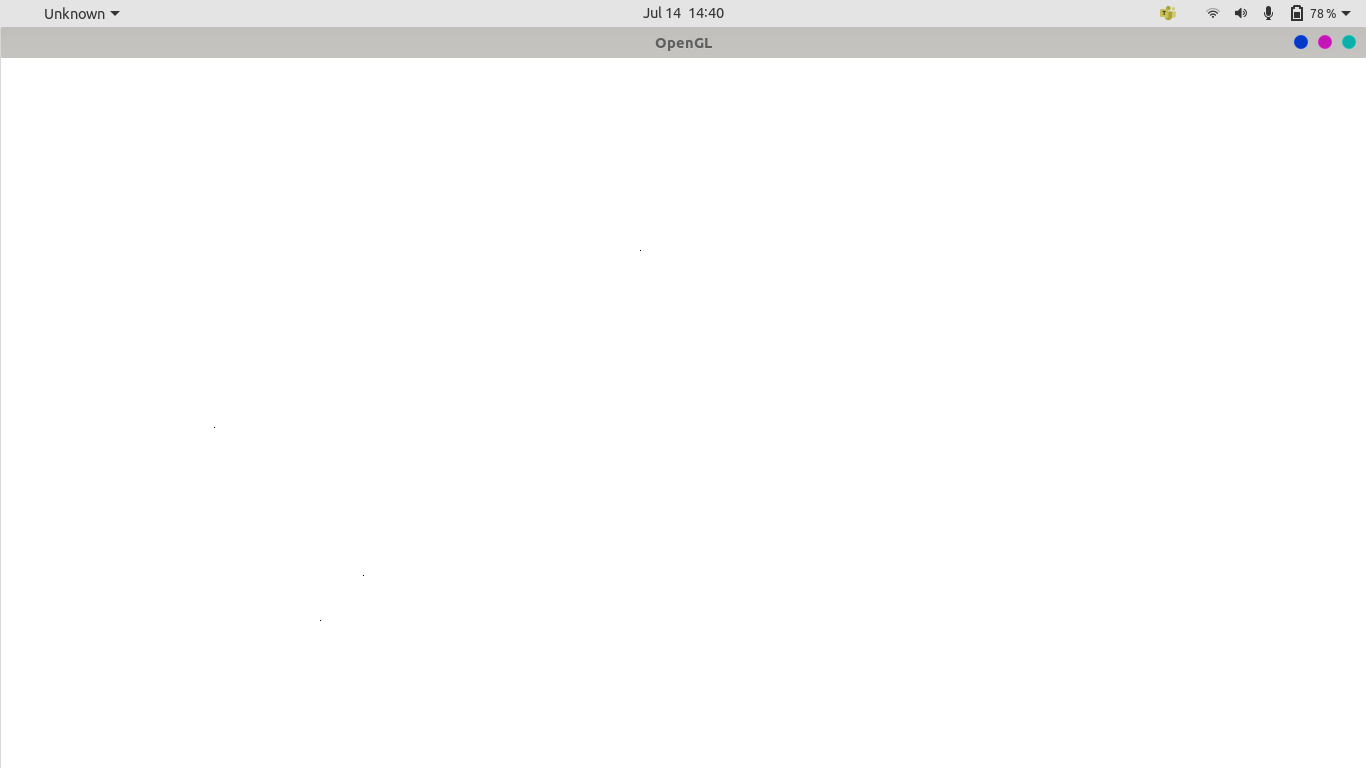
\includegraphics[height=8cm, keepaspectratio]{Basics/Outputs/Points.png}
\end{figure}

\newpage
\textbf{LINES:}
\lstinputlisting[language = C++, firstline=54, lastline=68]{./Basics/Helpers.h}
\textbf{\flushleft{Output:}}
\begin{figure}[h]
    \centering
    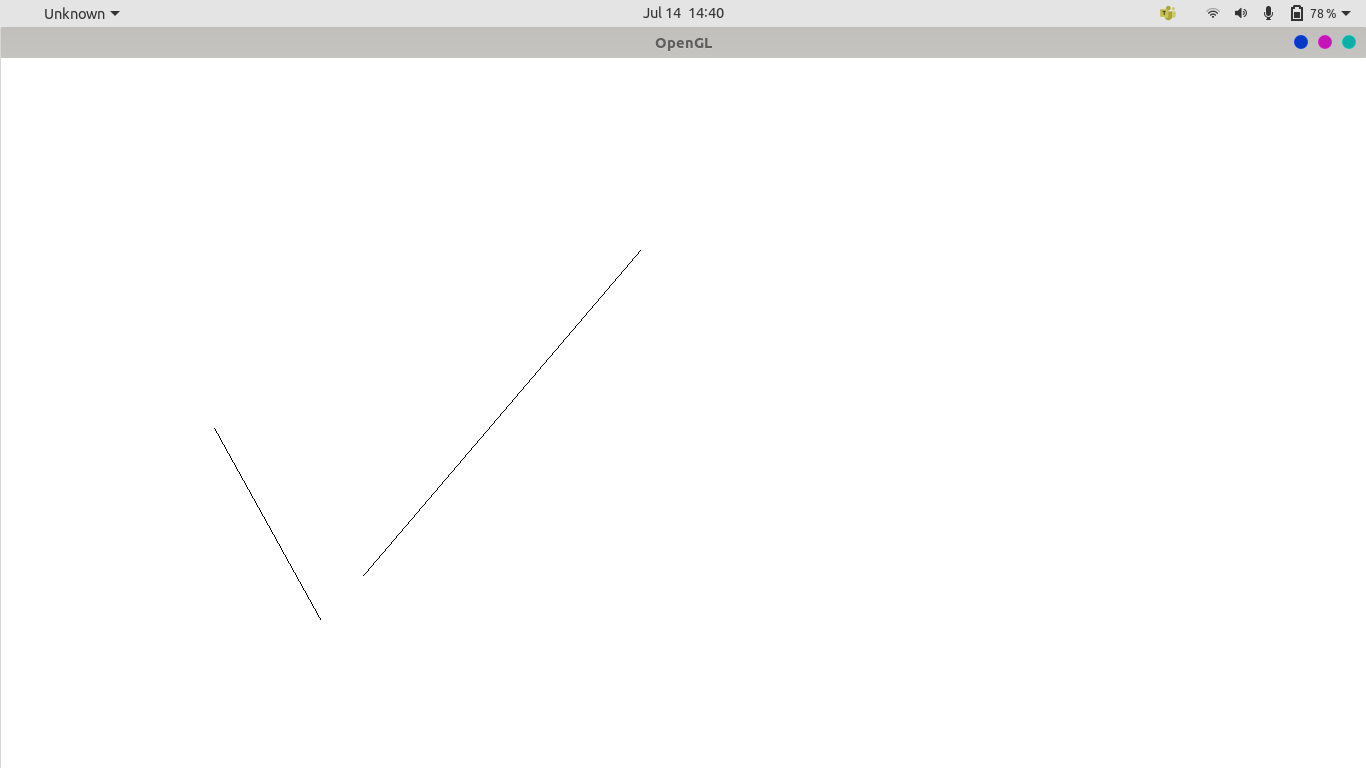
\includegraphics[height=8cm, keepaspectratio]{Basics/Outputs/Line.png}
\end{figure}

\newpage
\textbf{LINE\_STRIP:}
\lstinputlisting[language = C++, firstline=70, lastline=84]{./Basics/Helpers.h}
\textbf{\flushleft{Output:}}
\begin{figure}[h]
    \centering
    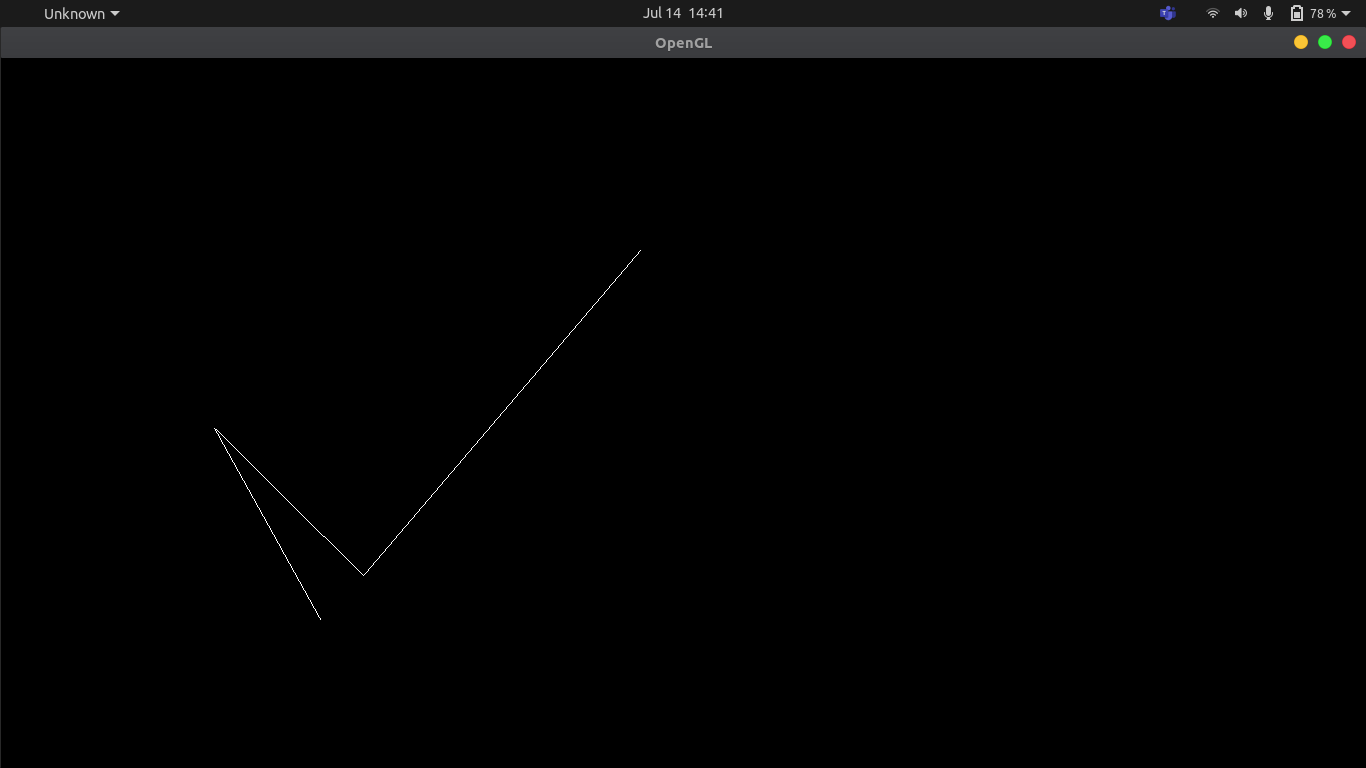
\includegraphics[height=8cm, keepaspectratio]{Basics/Outputs/Line_strip.png}
\end{figure}

\newpage
\textbf{LINE\_LOOP:}
\lstinputlisting[language = C++, firstline=86, lastline=100]{./Basics/Helpers.h}
\textbf{\flushleft{Output:}}
\begin{figure}[h]
    \centering
    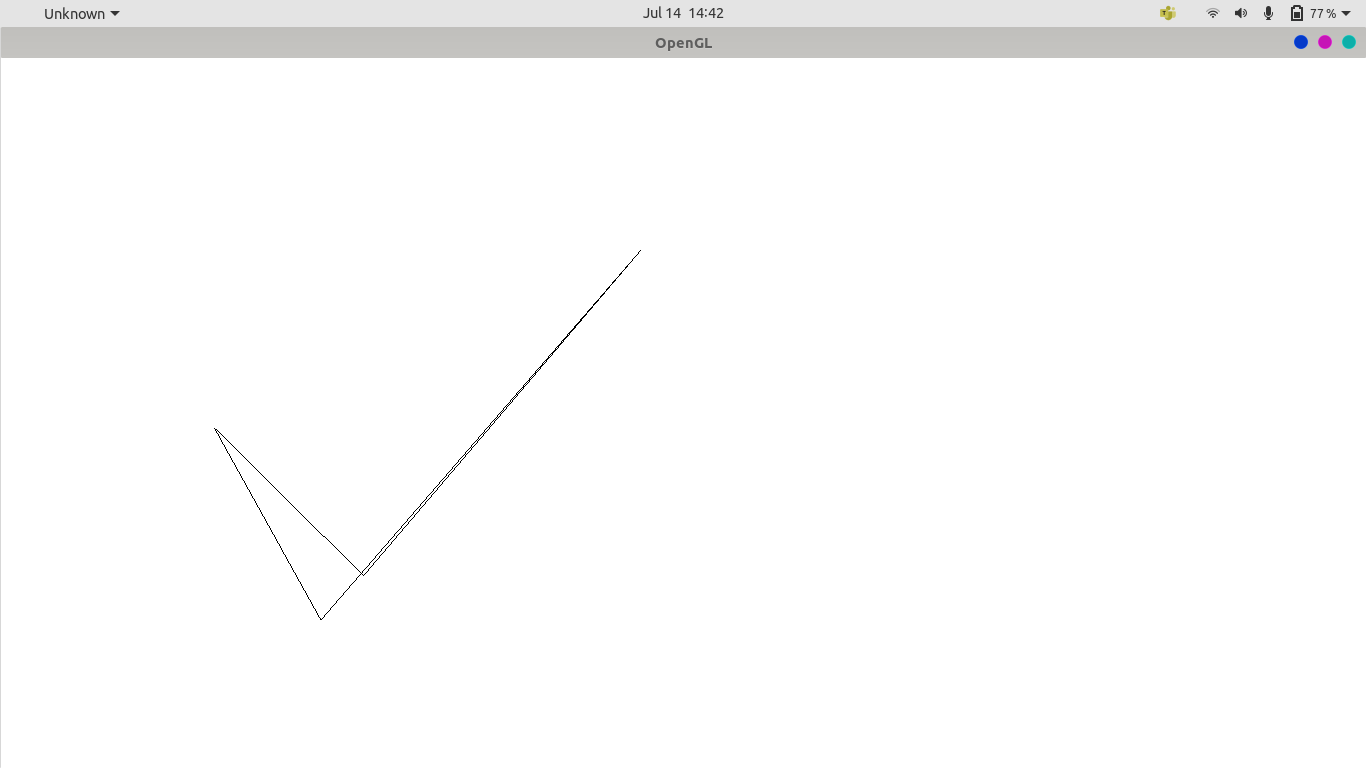
\includegraphics[height=8cm, keepaspectratio]{Basics/Outputs/Line_loop.png}
\end{figure}

\newpage
\textbf{TRIANGLES:}
\lstinputlisting[language = C++, firstline=102, lastline=116]{./Basics/Helpers.h}
\textbf{\flushleft{Output:}}
\begin{figure}[h]
    \centering
    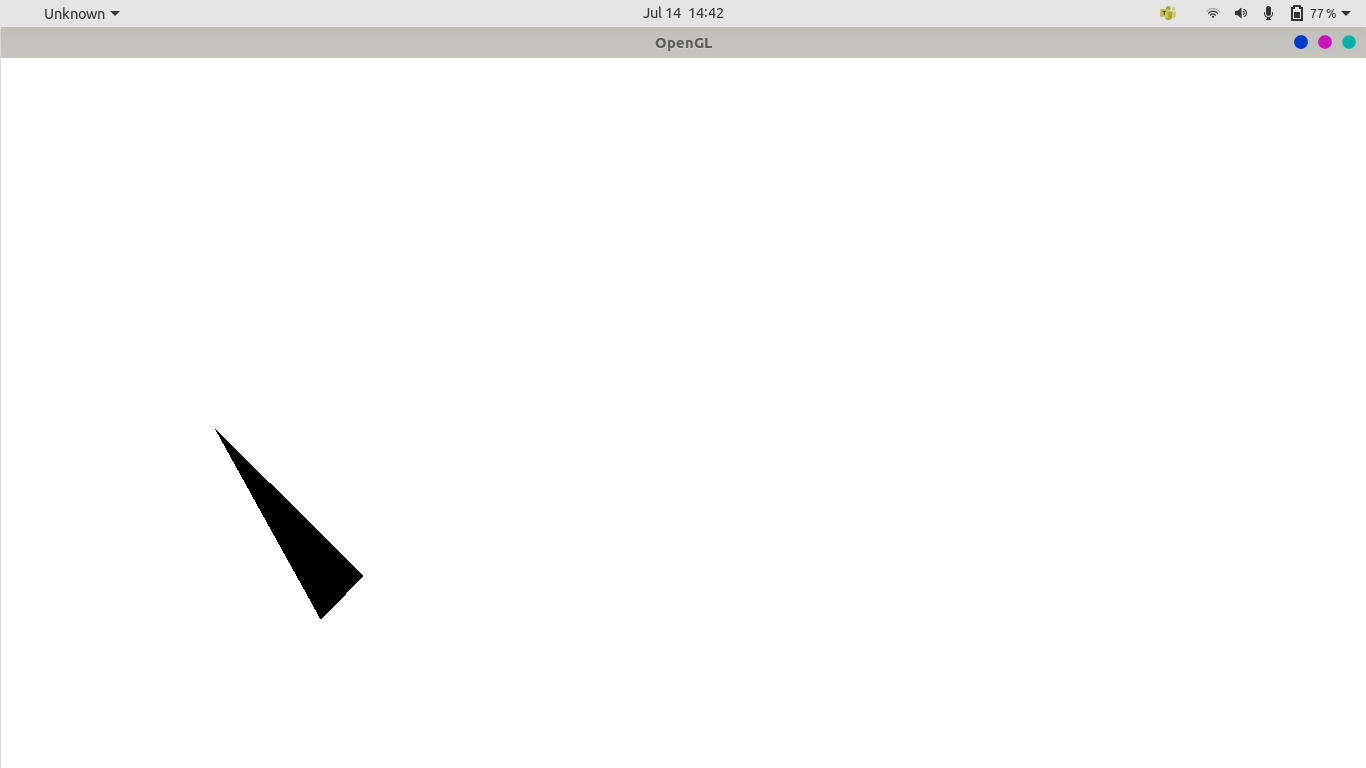
\includegraphics[height=8cm, keepaspectratio]{Basics/Outputs/Triangle.png}
\end{figure}

\newpage
\textbf{QUADS:}
\lstinputlisting[language = C++, firstline=118, lastline=132]{./Basics/Helpers.h}
\textbf{\flushleft{Output:}}
\begin{figure}[h]
    \centering
    
\includegraphics[height=8cm, keepaspectratio]{Basics/Outputs/Quad.png}
\end{figure}

\newpage
\textbf{QUAD\_STRIP:}
\lstinputlisting[language = C++, firstline=70, lastline=84]{./Basics/Helpers.h}
\textbf{\flushleft{Output:}}
\begin{figure}[h]
    \centering
    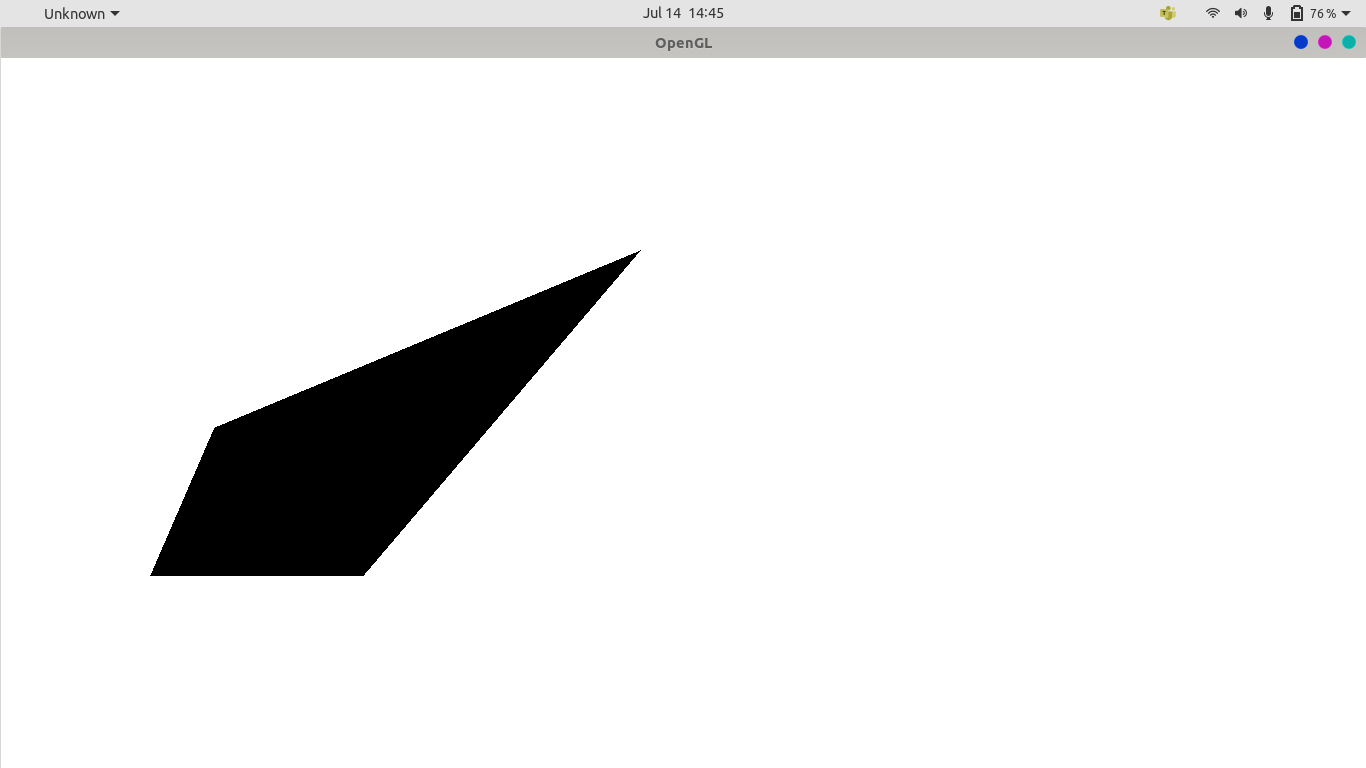
\includegraphics[height=8cm, keepaspectratio]{Basics/Outputs/Quad_strip.png}
\end{figure}

\newpage
\textbf{POLYGON:}
\lstinputlisting[language = C++, firstline=86, lastline=100]{./Basics/Helpers.h}
\textbf{\flushleft{Output:}}
\begin{figure}[h]
    \centering
    
\includegraphics[height=8cm, keepaspectratio]{Basics/Outputs/Polygon.png}
\end{figure}

\hrule
\bigskip\bigskip
\newpage
\subsection*{\flushleft{Aim:}}
\begin{flushleft}
    To create an output window and draw a checkerboard using OpenGL.    
\end{flushleft}

\subsection*{\flushleft{Code:}}
\begin{flushleft}
\lstinputlisting[language = C++]{./Chessboard/Headers.h}
\lstinputlisting[language = C++]{./Chessboard/Texture.h}
\lstinputlisting[language = C++]{./Chessboard/Texture.cpp}
\lstinputlisting[language = C++]{./Chessboard/Signatures.h}
\lstinputlisting[language = C++]{./Chessboard/Helpers.h}
\lstinputlisting[language = C++]{./Chessboard/main.cpp}
\end{flushleft}
\newpage
\subsection*{\flushleft{Output:}}
\begin{figure}[h]
    \centering
    
\includegraphics[height=8cm, keepaspectratio]{Chessboard/Outputs/Chessboard.png}
\end{figure}

\hrule
\bigskip\bigskip
\newpage
\subsection*{\flushleft{Aim:}}
\begin{flushleft}
    To create an output window and draw a house using POINTS,LINES,TRAINGLES and QUADS/POLYGON. 
\end{flushleft}

\subsection*{\flushleft{Code:}}
\begin{flushleft}
\lstinputlisting[language = C++]{House/Headers.h}
\lstinputlisting[language = C++]{House/Helpers.h}
\lstinputlisting[language = C++]{House/Signatures.h}
\lstinputlisting[language = C++]{House/main.cpp}
\end{flushleft}
% \newpage
\subsection*{\flushleft{Output:}}
\begin{figure}[h]
    \centering
    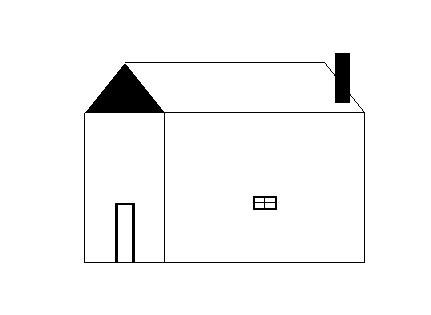
\includegraphics[height=8cm, keepaspectratio]{House/Outputs/house.png}
\end{figure}
\hrule

\end{document}